\documentclass[tikz,border=4pt]{standalone}
\usepackage[T1]{fontenc}
\usepackage[utf8]{inputenc}
\usepackage{amsmath,amssymb}
\usepackage{helvet}
\renewcommand{\familydefault}{\sfdefault}
\usepackage{pgfplots}
\pgfplotsset{compat=1.17}
\usetikzlibrary{arrows.meta,positioning,calc,fit,backgrounds,shapes.geometric}

\definecolor{cVis}{HTML}{1F77B4}
\definecolor{cTxt}{HTML}{D62728}
\definecolor{cProj}{HTML}{2CA02C}
\definecolor{cLLM}{HTML}{9467BD}
\definecolor{cConv}{HTML}{FF7F0E}
\definecolor{cAtt}{HTML}{17BECF}
\definecolor{cGray}{HTML}{7F7F7F}

\tikzset{
  blk/.style={draw, rounded corners=2pt, minimum height=8mm, align=center, font=\footnotesize, thick},
  tok/.style={draw, minimum size=3.2mm, inner sep=0pt},
  arr/.style={-{Stealth[length=2mm]}, thick},
}

\begin{document}
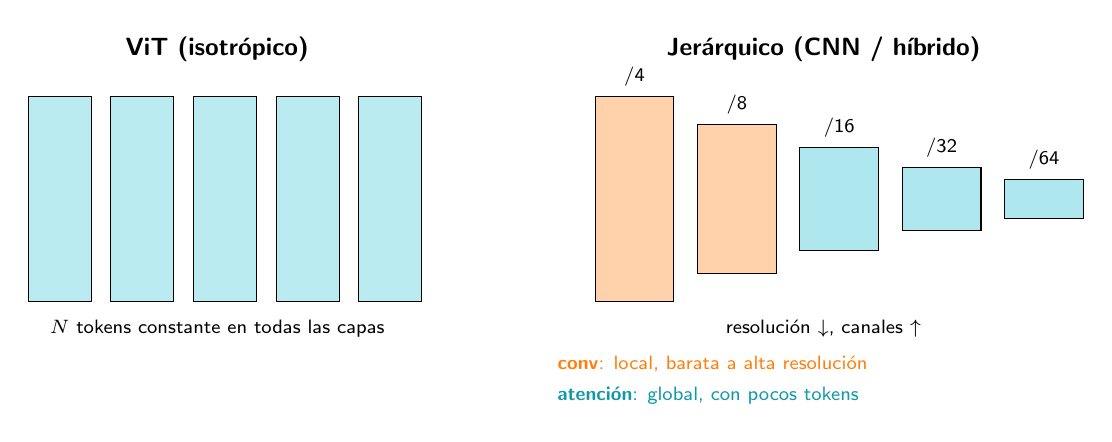
\begin{tikzpicture}[x=1cm,y=1cm]
  \node[font=\small\bfseries] at (2.4,3.2) {ViT (isotrópico)};
  \foreach \k in {0,...,4}{\draw[fill=cAtt!30] (\k*1.05,0) rectangle ++(0.8,2.6);}
  \node[font=\scriptsize] at (2.4,-0.35) {$N$ tokens constante en todas las capas};
  \node[font=\small\bfseries] at (10.1,3.2) {Jerárquico (CNN / híbrido)};
  \draw[fill=cConv!35] (7.2,0) rectangle ++(1.0,2.6);
  \draw[fill=cConv!35] (8.5,0.35) rectangle ++(1.0,1.9);
  \draw[fill=cAtt!35] (9.8,0.65) rectangle ++(1.0,1.3);
  \draw[fill=cAtt!35] (11.1,0.9) rectangle ++(1.0,0.8);
  \draw[fill=cAtt!35] (12.4,1.05) rectangle ++(1.0,0.5);
  \node[font=\scriptsize] at (7.7,2.85) {/4}; \node[font=\scriptsize] at (9.0,2.5) {/8};
  \node[font=\scriptsize] at (10.3,2.2) {/16}; \node[font=\scriptsize] at (11.6,1.95) {/32}; \node[font=\scriptsize] at (12.9,1.8) {/64};
  \node[font=\scriptsize] at (10.1,-0.35) {resolución $\downarrow$, canales $\uparrow$};
  \node[font=\scriptsize, text=cConv, anchor=west] at (6.6,-0.8) {\textbf{conv}: local, barata a alta resolución};
  \node[font=\scriptsize, text=cAtt!80!black, anchor=west] at (6.6,-1.2) {\textbf{atención}: global, con pocos tokens};
\end{tikzpicture}
\end{document}
